
%\documentclass[mathserif]{beamer}
\documentclass[handout]{beamer}
%\usetheme{Goettingen}
%\usetheme{Warsaw}
\usetheme{Singapore}



%\usetheme{Frankfurt}
%\usetheme{Copenhagen}
%\usetheme{Szeged}
%\usetheme{Montpellier}
%\usetheme{CambridgeUS}
%\usecolortheme{}
%\setbeamercovered{transparent}
\usepackage[english, activeacute]{babel}
\usepackage[utf8]{inputenc}
\usepackage{amsmath, amssymb}
\usepackage{dsfont}
\usepackage{graphics}
\usepackage{cases}
\usepackage{graphicx}
\usepackage{pgf}
\usepackage{epsfig}
\usepackage{amssymb}
\usepackage{multirow}	
\usepackage{amstext}
\usepackage[ruled,vlined,lined]{algorithm2e}
\usepackage{listings}
\usepackage{amsmath}
\usepackage{epic}
\usepackage{epsfig}
\usepackage{fontenc}
\usepackage{framed,color}
\usepackage{palatino, url, multicol}
%\algsetup{indent=2em}
\newcommand{\factorial}{\ensuremath{\mbox{\sc Factorial}}}
\newcommand{\BIGOP}[1]{\mathop{\mathchoice%
{\raise-0.22em\hbox{\huge $#1$}}%
{\raise-0.05em\hbox{\Large $#1$}}{\hbox{\large $#1$}}{#1}}}
\newcommand{\bigtimes}{\BIGOP{\times}}
\vspace{-0.5cm}
\title{Natural Language Processing \\ Sequence Labeling and Hidden Markov Models}
\vspace{-0.5cm}
\author[Felipe Bravo Márquez]{\footnotesize
%\author{\footnotesize  
 \textcolor[rgb]{0.00,0.00,1.00}{Felipe Bravo-Marquez}} 
  
 

\date{\today}

\begin{document}
\begin{frame}
\titlepage


\end{frame}



\begin{frame}{Overview}
  \scriptsize
  \begin{itemize}
    \item The Sequence Labeling (or Tagging) Problem
    \item Generative models, and the noisy-channel model, for supervised learning
    \item Hidden Markov Model (HMM) taggers
    \begin{itemize}\scriptsize
    \item Basic definitions
    \item Parameter estimation
    \item The Viterbi algorithm
    \end{itemize}
  \end{itemize}
 This slides are based on the course material by Michael Collins: \url{http://www.cs.columbia.edu/~mcollins/cs4705-spring2019/slides/tagging.pdf}

\end{frame}

\begin{frame}{Sequence Labeling or Tagging Tasks}

  \begin{itemize}
    \item Sequence Labeling or Tagging is a task in NLP different from document classification.
    \item Here the goal is to map a sentence represented as a sequence of tokens $x_1,x_2,\dots,x_n$ into a sequence of tags or labels $y_1,y_2,\dots,y_n$.
    \item Well known examples of this task are Part-of-Speech (POS) tagging and Named Entity Recognition (NER) to be presented next.
    \end{itemize}

\end{frame}




\begin{frame}
  \frametitle{Part-of-Speech Tagging}
  \scriptsize
  \textcolor{green}{\textbf{INPUT:}}
  Profits soared at Boeing Co., easily topping forecasts on Wall Street, as their CEO Alan Mulally announced first quarter results.  \vspace{0.5cm}
  
  \textcolor{green}{\textbf{OUTPUT:}}
  Profits\textcolor{red}{/N} soared\textcolor{red}{/V} at\textcolor{red}{/P} Boeing\textcolor{red}{/N} Co.\textcolor{red}{/N} ,\textcolor{red}{/,} easily\textcolor{red}{/ADV} topping\textcolor{red}{/V} forecasts\textcolor{red}{/N} on\textcolor{red}{/P} Wall\textcolor{red}{/N} Street\textcolor{red}{/N} ,\textcolor{red}{/,} as\textcolor{red}{/P} their\textcolor{red}{/POSS} CEO\textcolor{red}{/N} Alan\textcolor{red}{/N} Mulally\textcolor{red}{/N} announced\textcolor{red}{/V} first\textcolor{red}{/ADJ} quarter\textcolor{red}{/N} results\textcolor{red}{/N} .\textcolor{red}{/.}
   \vspace{0.5cm}
  \begin{itemize}
    \item \textcolor{red}{N} = \textcolor{blue}{Noun}
    \item \textcolor{red}{V} = \textcolor{blue}{Verb}
    \item \textcolor{red}{P} = \textcolor{blue}{Preposition}
    \item \textcolor{red}{Adv} = \textcolor{blue}{Adverb}
    \item \textcolor{red}{Adj} = \textcolor{blue}{Adjective}
    \item ...
  \end{itemize}
\end{frame}

\begin{frame}
  \frametitle{Named Entity Recognition}
  \textcolor{green}{\textbf{INPUT:}}
  Profits soared at Boeing Co., easily topping forecasts on Wall Street, as their CEO Alan Mulally announced first quarter results.    \vspace{0.5cm}

  \textcolor{green}{\textbf{OUTPUT:}}
  Profits soared at \textcolor{red}{[Company} Boeing Co.\textcolor{red}{]}, easily topping forecasts on \textcolor{red}{[Location} Wall Street\textcolor{red}{]}, as their CEO \textcolor{red}{[Person} Alan Mulally\textcolor{red}{]} announced first quarter results.
\end{frame}

\begin{frame}
  \frametitle{Named Entity Extraction as Sequence Labeling}
  \scriptsize
   \textcolor{green}{\textbf{INPUT:}}
  Profits soared at Boeing Co., easily topping forecasts on Wall Street, as their CEO Alan Mulally announced first quarter results. \vspace{0.5cm}

  \textcolor{green}{\textbf{OUTPUT:}}
  Profits\textcolor{red}{/NA} soared\textcolor{red}{/NA} at\textcolor{red}{/NA} Boeing\textcolor{purple}{/SC} Co.\textcolor{purple}{/CC} ,\textcolor{red}{/NA} easily\textcolor{red}{/NA} topping\textcolor{red}{/NA} forecasts\textcolor{red}{/NA} on\textcolor{red}{/NA} Wall\textcolor{purple}{/SL} Street\textcolor{purple}{/CL} ,\textcolor{red}{/NA} as\textcolor{red}{/NA} their\textcolor{red}{/NA} CEO\textcolor{red}{/NA} Alan\textcolor{purple}{/SP} Mulally\textcolor{purple}{/CP} announced\textcolor{red}{/NA} first\textcolor{red}{/NA} quarter\textcolor{red}{/NA} results\textcolor{red}{/NA} .\textcolor{red}{/NA} \vspace{0.5cm}

  \begin{itemize}
    \item \textcolor{red}{NA} = \textcolor{blue}{No entity}
    \item \textcolor{purple}{SC} = \textcolor{blue}{Start Company}
    \item \textcolor{purple}{CC} = \textcolor{blue}{Continue Company}
    \item \textcolor{purple}{SL} = \textcolor{blue}{Start Location}
    \item \textcolor{purple}{CL} = \textcolor{blue}{Continue Location}
    \item \textcolor{purple}{SP} = \textcolor{blue}{Start Person}
    \item \textcolor{purple}{CP} = \textcolor{blue}{Continue Person}
  \end{itemize}
\end{frame}


\begin{frame}
  \frametitle{Our Goal}
  \textbf{Training set:}
  \begin{enumerate}
    \item Pierre\textcolor{red}{/NNP} Vinken\textcolor{red}{/NNP} ,\textcolor{red}{/,} 61\textcolor{red}{/CD} years\textcolor{red}{/NNS} old\textcolor{red}{/JJ} ,\textcolor{red}{/,} will\textcolor{red}{/MD} join\textcolor{red}{/VB} the\textcolor{red}{/DT} board\textcolor{red}{/NN} as\textcolor{red}{/IN} a\textcolor{red}{/DT} nonexecutive\textcolor{red}{/JJ} director\textcolor{red}{/NN} Nov.\textcolor{red}{/NNP} 29\textcolor{red}{/CD} .\textcolor{red}{/.}
    \item Mr.\textcolor{red}{/NNP} Vinken\textcolor{red}{/NNP} is\textcolor{red}{/VBZ} chairman\textcolor{red}{/NN} of\textcolor{red}{/IN} Elsevier\textcolor{red}{/NNP} N.V.\textcolor{red}{/NNP} ,\textcolor{red}{/,} the\textcolor{red}{/DT} Dutch\textcolor{red}{/NNP} publishing\textcolor{red}{/VBG} group\textcolor{red}{/NN} .\textcolor{red}{/.}
    \item Rudolph\textcolor{red}{/NNP} Agnew\textcolor{red}{/NNP} ,\textcolor{red}{/,} 55\textcolor{red}{/CD} years\textcolor{red}{/NNS} old\textcolor{red}{/JJ} and\textcolor{red}{/CC} chairman\textcolor{red}{/NN} of\textcolor{red}{/IN} Consolidated\textcolor{red}{/NNP} Gold\textcolor{red}{/NNP} Fields\textcolor{red}{/NNP} PLC\textcolor{red}{/NNP} ,\textcolor{red}{/,} was\textcolor{red}{/VBD} named\textcolor{red}{/VBN} a\textcolor{red}{/DT} nonexecutive\textcolor{red}{/JJ} director\textcolor{red}{/NN} of\textcolor{red}{/IN} this\textcolor{red}{/DT} British\textcolor{red}{/JJ} industrial\textcolor{red}{/JJ} conglomerate\textcolor{red}{/NN} .\textcolor{red}{/.}
    \item ...
  \end{enumerate}

  \textbf{Our Goal:} From the training set, induce a function/algorithm that maps new sentences to their tag sequences.
\end{frame}

\begin{frame}
  \frametitle{Two Types of Constraints}
  Influential\textcolor{red}{/JJ} members\textcolor{red}{/NNS} of\textcolor{red}{/IN} the\textcolor{red}{/DT} House\textcolor{red}{/NNP} Ways\textcolor{red}{/NNP} and\textcolor{red}{/CC} Means\textcolor{red}{/NNP} Committee\textcolor{red}{/NNP} introduced\textcolor{red}{/VBD} legislation\textcolor{red}{/NN} that\textcolor{red}{/WDT} would\textcolor{red}{/MD} restrict\textcolor{red}{/VB} how\textcolor{red}{/WRB} the\textcolor{red}{/DT} new\textcolor{red}{/JJ} savings-and-loan\textcolor{red}{/NN} bailout\textcolor{red}{/NN} agency\textcolor{red}{/NN} can\textcolor{red}{/MD} raise\textcolor{red}{/VB} capital\textcolor{red}{/NN} .\textcolor{red}{/.} \vspace{0.5cm}

  \textbf{``Local'':}
  \begin{itemize}
    \item e.g., ``can'' is more likely to be a modal verb \textcolor{red}{MD} rather than a noun \textcolor{red}{NN}
  \end{itemize}

  \textbf{``Contextual'':}
  \begin{itemize}
    \item e.g., a noun is much more likely than a verb to follow a determiner
  \end{itemize}

  \textbf{Sometimes these preferences are in conflict:}
  \begin{itemize}
    \item The trash can is in the garage
  \end{itemize}
\end{frame}


\begin{frame}
  \frametitle{Sequence Labeling as Supervised Learning}

    \begin{itemize}
      \item We have a sequence of inputs $x = (x_1, x_2, \ldots, x_n)$ and corresponding labels $y = (y_1, y_2, \ldots, y_n)$.
      \item Task is to learn a function $f$ that maps input sequences to label sequences: $f(x_1,x_2, \ldots, x_n) = y_1, y_2, \ldots, y_n$.
      \item We have a training set of labeled sequences: $\{(x^{(1)}, y^{(1)}), (x^{(2)}, y^{(2)}), \ldots, (x^{(m)}, y^{(m)})\}$.
    \end{itemize}
  
\end{frame}

\begin{frame}
  \frametitle{Generative Approach for Sequence Labeling}
  \scriptsize
  \begin{itemize}
    \item Generative models such as Naive Bayes was used for classification can also be used for sequence labeling tasks in NLP.
    \item Approach:
    \begin{itemize}\scriptsize
      \item Training: Learn the joint distribution $p(x_1,x_2, \ldots, x_n,y_1, y_2, \ldots, y_n)$ of input sequences.
      \item Decoding: Use the learned distribution to predict label sequences for new input sequences.
    \end{itemize}
      \item Decoding in sequence labeling involves finding the label sequence with the highest joint probability: $\arg\max_{y_1, y_2, \ldots, y_n}p(x_1,x_2, \ldots, x_n,y_1, y_2, \ldots, y_n)$.
  \end{itemize}
\end{frame}






\begin{frame}
  \frametitle{Hidden Markov Models}
  \scriptsize
  \begin{itemize}
    \item  Hidden Markov Models (HMMs) provide a principled way to handle sequence labeling problems using generative modeling and efficient decoding algorithms.
    \item We have an input sentence $x = x_1, x_2, \ldots, x_n$ ($x_i$ is the $i$-th word in the sentence).
    \item We have a tag sequence $y = y_1, y_2, \ldots, y_n$ ($y_i$ is the $i$-th tag in the sentence).
    \item We'll use an HMM to define $p(x_1, x_2, \ldots, x_n, y_1, y_2, \ldots, y_n)$ for any sentence $x_1, \ldots, x_n$ and tag sequence $y_1, \ldots, y_n$ of the same length. \cite{kupiec1992robust}
    \item Then, the most likely tag sequence for $x$ is:
    \[
      \arg\max_{y_1,\ldots,y_n} p(x_1, \ldots, x_n, y_1, \ldots, y_n)
    \]
  \end{itemize}
\end{frame}

\begin{frame}
  \frametitle{Trigram Hidden Markov Models (Trigram HMMs)}
  For any sentence $x_1, \ldots, x_n$ where $x_i \in V$ for $i = 1, \ldots, n$, and any tag sequence $y_1, \ldots, y_{n+1}$ where $y_i \in S$ for $i = 1, \ldots, n$, and $y_{n+1} = \text{STOP}$, the joint probability of the sentence and tag sequence is:
  \[
    p(x_1, \ldots, x_n, y_1, \ldots, y_{n+1}) = \prod_{i=1}^{n+1} q(y_i | y_{i-2}, y_{i-1}) \prod_{i=1}^{n} e(x_i | y_i)
  \]
  where we have assumed that $x_0 = x_{-1} = *$.
\end{frame}

\begin{frame}
  \frametitle{Parameters of the Model}
  \begin{itemize}
    \item $q(s|u, v)$ for any $s \in S \cup \{\text{STOP}\}$, $u, v \in S \cup \{*\}$
    \item $e(x|s)$ for any $s \in S$, $x \in V$
  \end{itemize}
\end{frame}

\begin{frame}
  \frametitle{An Example}
  \scriptsize
  If we have $n = 3$, $x_1, x_2, x_3$ equal to the sentence "the dog laughs", and $y_1, y_2, y_3, y_4$ equal to the tag sequence "D N V STOP", then:
\[
\begin{aligned}
p(x_1, \ldots, x_n, y_1, \ldots, y_{n+1}) = & q(D|*,*) \times q(N|*,D) \\
& \times q(V|D,N) \times q(\text{STOP}|N,V) \\
& \times e(\text{the}|D) \times e(\text{dog}|N) \times e(\text{laughs}|V)
\end{aligned}
\]
  \begin{itemize}
    \item STOP is a special tag that terminates the sequence.
    \item We take $y_0 = y_{-1} = *$, where $*$ is a special "padding" symbol.
  \end{itemize}
\end{frame}

\begin{frame}
  \frametitle{Why the Name?}
\[
\begin{aligned}
p(x_1, \ldots, x_n, y_1, \ldots, y_n) = & q(\text{STOP}|y_{n-1}, y_n) \\
& \times \prod_{j=1}^{n} q(y_j | y_{j-2}, y_{j-1}) \\
& \times \prod_{j=1}^{n} e(x_j | y_j)
\end{aligned}
\]
  \begin{itemize}
    \item Markov Chain:
    \[
      q(\text{STOP}|y_{n-1}, y_n)\times \prod_{j=1}^{n} q(y_j | y_{j-2}, y_{j-1})
    \]
    \item Observed:
    \[
      e(x_j | y_j)
    \]
  \end{itemize}
\end{frame}



\begin{frame}
\frametitle{Smoothed Estimation}

\[
\begin{aligned}
q(Vt | DT, JJ) = & \lambda_1 \times \frac{{\text{Count}(Dt, JJ, Vt)}}{{\text{Count}(Dt, JJ)}} \\
& + \lambda_2 \times \frac{{\text{Count}(JJ, Vt)}}{{\text{Count}(JJ)}} \\
& + \lambda_3 \times \frac{{\text{Count}(Vt)}}{{\text{Count}()}}
\end{aligned}
\]

where $\lambda_1 + \lambda_2 + \lambda_3 = 1$, and for all $i$, $\lambda_i \geq 0$.

\vspace{0.5cm}

\[
e(\text{base} | Vt) = \frac{{\text{Count}(Vt, \text{base})}}{{\text{Count}(Vt)}}
\]

\end{frame}

\begin{frame}
\frametitle{Dealing with Low-Frequency Words}

A common method is as follows:
\begin{itemize}
  \item Step 1: Split vocabulary into two sets
    \begin{itemize}
      \item Frequent words = words occurring $\geq 5$ times in training
      \item Low frequency words = all other words
    \end{itemize}
  \item Step 2: Map low frequency words into a small, finite set, depending on prefixes, suffixes, etc.
\end{itemize}

\end{frame}



\begin{frame}
  \frametitle{Dealing with Low-Frequency Words: An Example}
  \scriptsize
  
 Below is an example of word classes for named entity recognition \cite{bikelSW99}:
  
  \[
    \begin{array}{l|l|l}
      \text{Word class} & \text{Example}  & \text{Intuition} \\
      \hline
      \text{twoDigitNum} & 90 & \text{Two-digit year} \\
      \text{fourDigitNum} & 1990 & \text{Four-digit year} \\
      \text{containsDigitAndAlpha} & A8956-67 & \text{Product code} \\
      \text{containsDigitAndDash} & 09-96 & \text{Date} \\
      \text{containsDigitAndSlash} & 11/9/89 & \text{Date} \\
      \text{containsDigitAndComma} & 23,000.00 & \text{Monetary amount} \\
      \text{containsDigitAndPeriod} & 1.00 & \text{Monetary amount, percentage} \\
      \text{othernum} & 456789 & \text{Other number} \\
      \text{allCaps} & BBN & \text{Organization} \\
      \text{capPeriod} & M. & \text{Person name initial} \\
      \text{firstWord} & \text{First word of sentence} & \text{No useful capitalization information} \\
      \text{initCap} & \text{Sally} & \text{Capitalized word} \\
      \text{lowercase} & \text{can} & \text{Uncapitalized word} \\
      \text{other} & , & \text{Punctuation marks, all other words} \\
    \end{array}
  \]
\end{frame}

\begin{frame}
  \frametitle{Dealing with Low-Frequency Words: An Example}
  \scriptsize
  
  
\textbf{Original Sentence:}

  Profits\textcolor{red}{/NA} soared\textcolor{red}{/NA} at\textcolor{red}{/NA} Boeing\textcolor{purple}{/SC} Co.\textcolor{purple}{/CC} ,\textcolor{red}{/NA} easily\textcolor{red}{/NA} topping\textcolor{red}{/NA} forecasts\textcolor{red}{/NA} on\textcolor{red}{/NA} Wall\textcolor{purple}{/SL} Street\textcolor{purple}{/CL} ,\textcolor{red}{/NA} as\textcolor{red}{/NA} their\textcolor{red}{/NA} CEO\textcolor{red}{/NA} Alan\textcolor{purple}{/SP} Mulally\textcolor{purple}{/CP} announced\textcolor{red}{/NA} first\textcolor{red}{/NA} quarter\textcolor{red}{/NA} results\textcolor{red}{/NA} .\textcolor{red}{/NA} \vspace{0.5cm}


\textbf{Transformed Sentence:}

firstword\textcolor{red}{/NA} soared\textcolor{red}{/NA} at\textcolor{red}{/NA} initCap\textcolor{purple}{/SC} Co.\textcolor{purple}{/CC} ,\textcolor{red}{/NA} easily\textcolor{red}{/NA} lowercase\textcolor{red}{/NA} forecasts\textcolor{red}{/NA} on\textcolor{red}{/NA} initCap\textcolor{purple}{/SL} Street\textcolor{purple}{/CL} ,\textcolor{red}{/NA} as\textcolor{red}{/NA} their\textcolor{red}{/NA} CEO\textcolor{red}{/NA} Alan\textcolor{purple}{/SP} initCap\textcolor{purple}{/CP} announced\textcolor{red}{/NA} first\textcolor{red}{/NA} quarter\textcolor{red}{/NA} results\textcolor{red}{/NA} .\textcolor{red}{/NA} \vspace{0.5cm}


  \begin{itemize}
    \item \textcolor{red}{NA} = \textcolor{blue}{No entity}
    \item \textcolor{purple}{SC} = \textcolor{blue}{Start Company}
    \item \textcolor{purple}{CC} = \textcolor{blue}{Continue Company}
    \item \textcolor{purple}{SL} = \textcolor{blue}{Start Location}
    \item \textcolor{purple}{CL} = \textcolor{blue}{Continue Location}
    \item \textcolor{purple}{SP} = \textcolor{blue}{Start Person}
    \item \textcolor{purple}{CP} = \textcolor{blue}{Continue Person}
  \end{itemize}
\end{frame}






\begin{frame}[fragile]
  \frametitle{Dynamic Programming}

  \begin{itemize}
    \item Dynamic programming is a technique used to solve optimization problems by breaking them down into overlapping subproblems.
    \item It stores the solutions to these subproblems in a table, so they do not need to be recalculated.
    \item Dynamic programming can greatly improve the efficiency of algorithms.
  \end{itemize}

\end{frame}

\begin{frame}[fragile]
  \frametitle{Factorial}

  \begin{itemize}
    \item Recursive implementation:

    \begin{lstlisting}[language=Python]
def recur_factorial(n):
    # Base case
    if n == 1:
        return n
    else:
        return n * recur_factorial(n-1)
    \end{lstlisting}

    \item Dynamic programming implementation:

    \begin{lstlisting}[language=Python]
def dynamic_factorial(n):
    table = [0 for i in range(0, n+1)]

    # Base case
    table[0] = 1

    for i in range(1, len(table)):
        table[i] = i * table[i-1]

    return table[n]
    \end{lstlisting}

  \end{itemize}

\end{frame}

\begin{frame}[fragile]
  \frametitle{Fibonacci}

  \begin{itemize}
    \item Recursive implementation:

    \begin{lstlisting}[language=Python]
def recur_fibonacci(n):
    if n == 1 or n == 0:
        return 1
    else:
        return recur_fibonacci(n-1) + recur_fibonacci(n-2)
    \end{lstlisting}

    \item Dynamic programming implementation:

    \begin{lstlisting}[language=Python]
def dynamic_fibonacci(n):
    table = [0 for i in range(0, n+1)]

    # Base case
    table[0] = 1
    table[1] = 1

    for i in range(2, len(table)):
        table[i] = table[i-1] + table[i-2]

    return table[n]
    \end{lstlisting}

  \end{itemize}

\end{frame}

\begin{frame}
  \frametitle{Complexity}

  \begin{itemize}
    \item Recursive factorial: Exponential complexity
    \item Dynamic factorial: Linear complexity
    \item Recursive Fibonacci: Exponential complexity
    \item Dynamic Fibonacci: Linear complexity
  \end{itemize}

\end{frame}




\begin{frame}
  \frametitle{The Viterbi Algorithm}
  Problem: For an input $x_1 \ldots x_n$, find
  \[
    \arg \max_{y_1 \ldots y_{n+1}} p(x_1 \ldots x_n, y_1 \ldots y_{n+1})
  \]
  where the $\arg \max$ is taken over all sequences $y_1 \ldots y_{n+1}$ such that $y_i \in S$ for $i = 1 \ldots n$, and $y_{n+1} = \text{STOP}$.

  We assume that $p$ takes the form:
  \[
    p(x_1 \ldots x_n, y_1 \ldots y_{n+1}) = \prod_{i=1}^{n+1} q(y_i|y_{i-2}, y_{i-1}) \prod_{i=1}^{n} e(x_i|y_i)
  \]
\end{frame}

\begin{frame}
  \frametitle{Brute Force Search is Hopelessly Inefficient}
  Problem: For an input $x_1 \ldots x_n$, find
  \[
    \arg \max_{y_1 \ldots y_{n+1}} p(x_1 \ldots x_n, y_1 \ldots y_{n+1})
  \]
  where the $\arg \max$ is taken over all sequences $y_1 \ldots y_{n+1}$ such that $y_i \in S$ for $i = 1 \ldots n$, and $y_{n+1} = \text{STOP}$.
\end{frame}

\begin{frame}
  \frametitle{The Viterbi Algorithm}
  The Viterbi algorithm efficiently computes the maximum probability of a tag sequence by using dynamic programming.

  \textbf{Steps:}
  \begin{itemize}
    \item Define $n$ as the length of the sentence.
    \item Define $S_k$ for $k = -1 \ldots n$ as the set of possible tags at position $k$: $S_{-1} = S_0 = \{*\}$, $S_k = S$ for $k \in \{1 \ldots n\}$.
    \item Define $r(y_{-1}, y_0, y_1, \ldots, y_k) = \prod_{i=1}^k q(y_i|y_{i-2}, y_{i-1}) \prod_{i=1}^k e(x_i|y_i)$.
    \item Define a dynamic programming table: $\pi(k, u, v)$ = maximum probability of a tag sequence ending in tags $u$, $v$ at position $k$.
  \end{itemize}
\end{frame}

\begin{frame}
  \frametitle{An Example}
  $\pi(k, u, v)$ = maximum probability of a tag sequence ending in tags $u$, $v$ at position $k$

  \textbf{The man saw the dog with the telescope}




\end{frame}


\begin{frame}
  \frametitle{An Example}

  \begin{figure}[h]
        	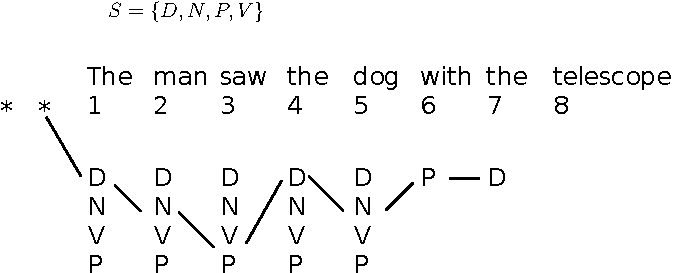
\includegraphics[scale = 0.7]{pics/viterbi1.pdf}
        \end{figure}



\end{frame}

\begin{frame}
  \frametitle{A Recursive Definition}
  \textbf{Base case:}
  \[
    \pi(0, *, *) = 1
  \]

  \textbf{Recursive definition:}
  For any $k \in \{1 \ldots n\}$, for any $u \in S_{k-1}$ and $v \in S_k$:
  \[
    \pi(k, u, v) = \max_{w \in S_{k-2}} (\pi(k - 1, w, u) \times q(v|w, u) \times e(x_k|v))
  \]
\end{frame}

\begin{frame}
  \frametitle{Justification for the Recursive Definition}
  For any $k \in \{1 \ldots n\}$, for any $u \in S_{k-1}$ and $v \in S_k$:
  \[
    \pi(k, u, v) = \max_{w \in S_{k-2}} (\pi(k - 1, w, u) \times q(v|w, u) \times e(x_k|v))
  \]

  \textbf{The man saw the dog with the telescope}
\end{frame}


\begin{frame}
  \frametitle{Justification for the Recursive Definition}

  \begin{figure}[h]
        	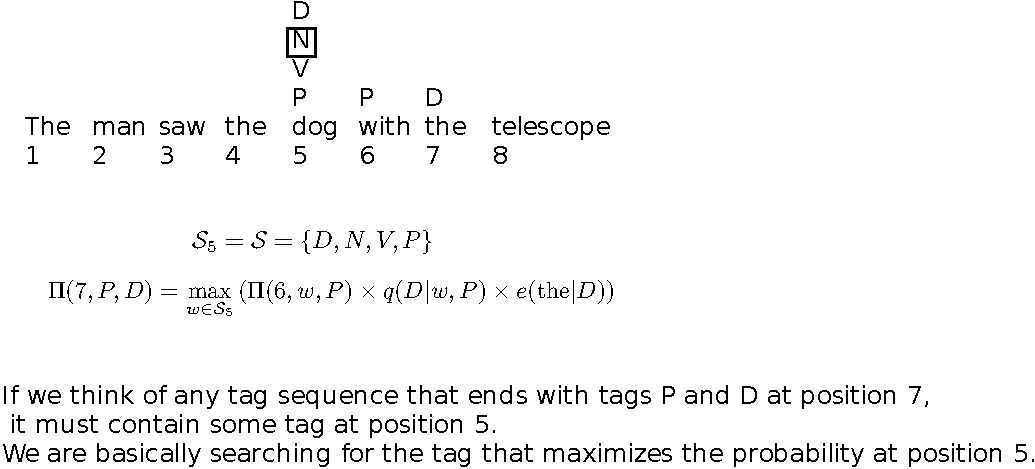
\includegraphics[scale = 0.65]{pics/viterbi2.pdf}
        \end{figure}
\end{frame}

\begin{frame}
  \frametitle{The Viterbi Algorithm}
\begin{algorithm}[H]
\SetKwInput{Input}{Input}
\SetKwInput{Initialization}{Initialization}
\SetKwFunction{Max}{max}
\SetKwFunction{Return}{return}

\Input{a sentence $x_1 \ldots x_n$, parameters $q(s|u, v)$ and $e(x|s)$}

\Initialization{ Set $\pi(0, *, *) = 1$;  $S_{-1} = S_0 = \{*\}$, $S_k = S$ for $k \in \{1 \ldots n\}$.
}

\BlankLine
\SetAlgoLined
\caption{Viterbi Algorithm}
\label{algo:prob_inference}
\BlankLine

\For{$k = 1$ \KwTo $n$}{
\For{$u \in S_{k-1}, v \in S_k$}{\[\pi(k, u, v) = \max_{w \in S_{k-2}} (\pi(k - 1, w, u) \times q(v|w, u) \times e(x_k|v))\]} 
}



\BlankLine
\Return{$\max_{u \in S_{n-1}, v \in S_n} (\pi(n, u, v) \times q(\text{STOP}|u, v))$} 
\end{algorithm}
\end{frame}



\begin{frame}{The Viterbi Algorithm with Backpointers}
\scriptsize
\begin{algorithm}[H]
\SetKwInput{Input}{Input}
\SetKwInput{Initialization}{Initialization}
\SetKwFunction{Max}{max}
\SetKwFunction{ArgMax}{argmax}
\SetKwFunction{Return}{return}

\Input{a sentence $x_1 \ldots x_n$, parameters $q(s|u, v)$ and $e(x|s)$}

\Initialization{Set $\pi(0, *, *) = 1$;  $S_{-1} = S_0 = \{*\}$, $S_k = S$ for $k \in \{1 \ldots n\}$.
}

\BlankLine
\SetAlgoLined
\caption{Viterbi Algorithm with Backpointers}
\label{algo:viterbi}
\BlankLine

\For{$k = 1$ \KwTo $n$}{
\For{$u \in S_{k-1}, v \in S_k$}{
\[
\pi(k, u, v) = \max_{w \in S_{k-2}} (\pi(k - 1, w, u) \times q(v|w, u) \times e(x_k|v))
\]    
\[
\text{bp}(k, u, v) = \arg \max_{w \in S_{k-2}} (\pi(k - 1, w, u) \times q(v|w, u) \times e(x_k|v))
    \]} 
}



\BlankLine
$(y_{n-1}, y_n) = \arg \max_{(u,v)} (\pi(n, u, v) \times q(\text{STOP}|u, v))$ \tcp*[r]{Find maximum probability and corresponding tags}
\For{$k = (n - 2)$ \KwTo $1$}{
$y_k = \text{bp}(k + 2, y_{k+1}, y_{k+2})$ \tcp*[r]{Retrieve tag sequence using backpointers}
}

\BlankLine
\Return{the tag sequence $y_1 \ldots y_n$} \tcp*[r]{Return the final tag sequence}
\end{algorithm}
\end{frame}



\begin{frame}
  \frametitle{The Viterbi Algorithm: Running Time}
  \begin{itemize}
    \item $O(n|S|^3)$ time to calculate $q(s|u, v) \times e(x_k|s)$ for all $k, s, u, v$.
    \item $n|S|^2$ entries in $\pi$ to be filled in.
    \item $O(|S|)$ time to fill in one entry.
  \end{itemize}
  $\Rightarrow$ $O(n|S|^3)$ time in total.
\end{frame}

\begin{frame}
  \frametitle{Pros and Cons}
  \begin{itemize}
    \item Hidden Markov Model (HMM) taggers are simple to train (compile counts from training corpus).
    \item They perform relatively well (over 90% performance on named entity recognition).
    \item Main difficulty is modeling $e(\text{word} | \text{tag})$, which can be very complex if "words" are complex.
  \end{itemize}
\end{frame}


\begin{frame}
\frametitle{Questions?}
%\vspace{1.5cm}
\begin{center}\LARGE Thanks for your Attention!\\ \end{center}



\end{frame}

\begin{frame}[allowframebreaks]\scriptsize
\frametitle{References}
\bibliography{bio}
\bibliographystyle{apalike}
%\bibliographystyle{flexbib}
\end{frame}  


%%%%%%%%%%%%%%%%%%%%%%%%%%%

\end{document}
